\section{Qualitätsanforderungen}

Dieses Kapitel beschreibt die nichtfunktionalen Anforderungen an EduPlanner anhand von ISO/IEC~25010 Qualitätskategorien. Die Anforderungen werden zunächst als hierarchischer Qualitätsbaum strukturiert und anschließend in messbaren Szenarien konkretisiert, die als Grundlage für Architekturentscheidungen und Akzeptanztests dienen.

\subsection{Qualitätsbaum}

Der Qualitätsbaum (arc42~v9: Pflicht) gibt eine hierarchische Übersicht aller relevanten Qualitätseigenschaften von EduPlanner, gegliedert nach ISO/IEC~25010 Hauptkategorien. Er dient als Navigation in die konkreten Szenarien in Kap.~10.2 und ermöglicht die schnelle Priorisierung im ATAM-light-Prozess.

\begin{figure}[H]
  \centering
  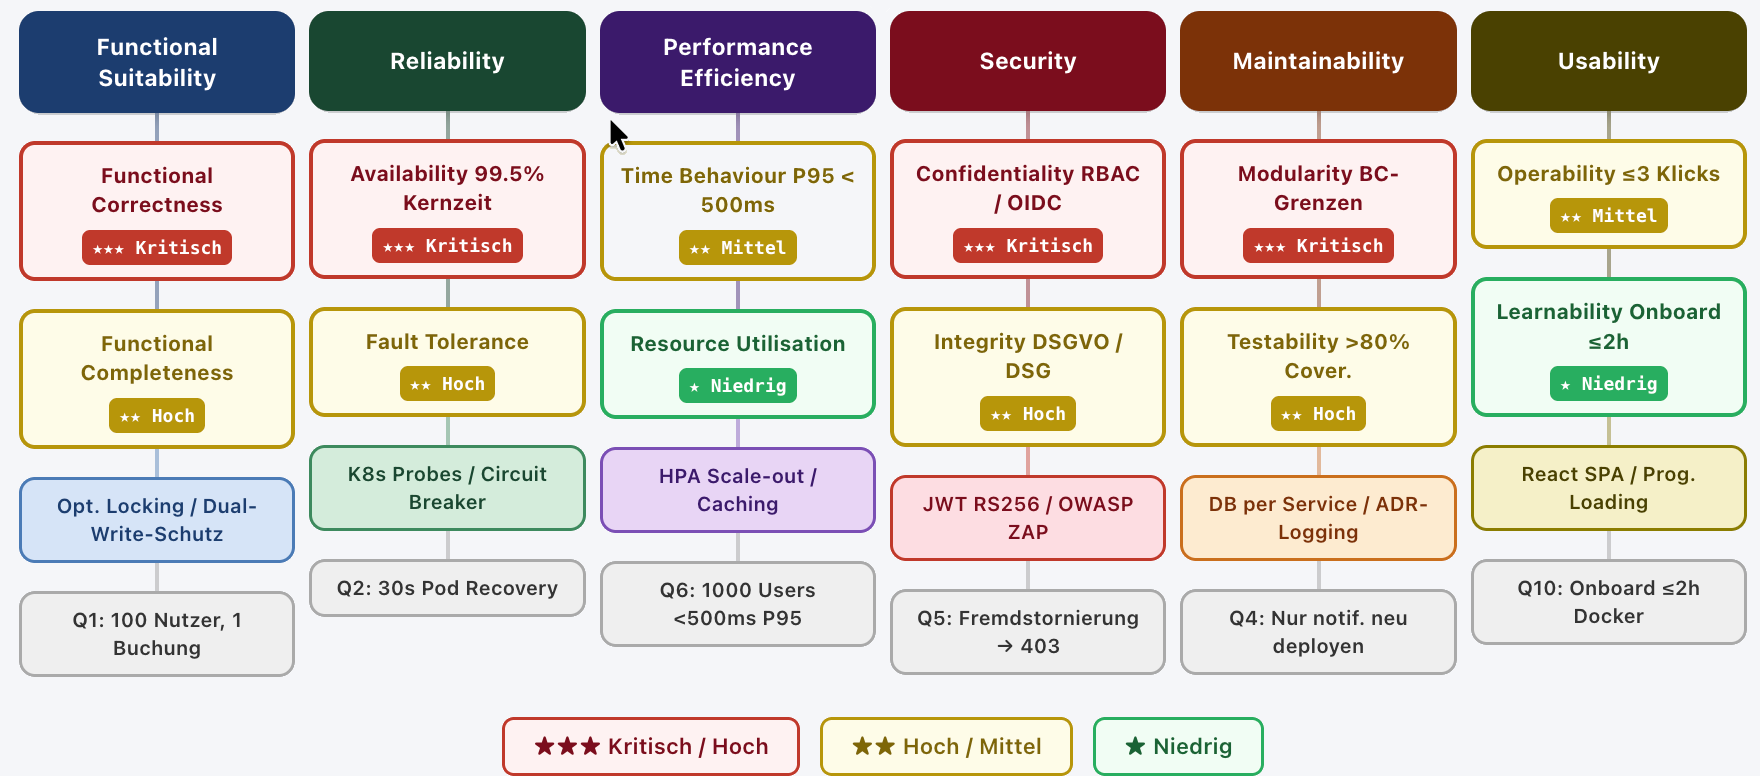
\includegraphics[width=\textwidth]{assets/QualityTree}
  \caption{\textit{Qualitätsbaum: EduPlanner Qualitätsanforderungen}}
  \label{fig:QualityTree}
\end{figure}

\textbf{ATAM-light -- Wesentliche Trade-offs in EduPlanner:}\footnote{%
  \textit{Architecture Tradeoff Analysis Method (ATAM):} Strukturierte Methode zur Architekturbewertung,
  die konkurrierende Qualitätsziele systematisch analysiert und Trade-offs explizit macht.
  „ATAM-light" bezeichnet hier eine vereinfachte, projektangepasste Variante ohne vollständigen ATAM-Workshop.}

\begin{description}[leftmargin=0pt, style=nextline]

  \item[Microservices (ADR-001):
    $\uparrow$~Maintainability,\;$\uparrow$~Scalability,\;$\downarrow$~Betriebskomplexität]
  Jeder Bounded Context wird als eigenständiger Service deployt.
  \textit{Gewinn:} Ein Team kann den \texttt{registration}-Service ändern und deployen,
  ohne dass andere Services neu gestartet werden müssen -- das erhöht die
  Wartbarkeit erheblich. Ausserdem kann der \texttt{registration}-Service zur
  Einschreibungsfrist auf 10~Pods hochskaliert werden, während
  \texttt{catalog} bei 1~Pod bleibt.
  \textit{Preis:} Das System besteht nun aus fünf laufenden Prozessen, fünf
  Datenbanken, einem Message Broker und einem API Gateway -- all das muss
  überwacht, gepatcht und betrieben werden. Ein Entwickler, der lokal arbeitet,
  startet nicht mehr eine Applikation, sondern eine ganze Landschaft via Docker
  Compose. Dieser Overhead ist das bewusst eingegangene Risiko für die
  gewonnene Unabhängigkeit (vgl.\ Risiko R5).

  \item[Asynchrones Messaging (ADR-002):
    $\uparrow$~Availability,\;$\uparrow$~Maintainability,\;$\downarrow$~Eventual Consistency]
  Zustandsändernde Ereignisse zwischen Services (z.\,B.\ ``Teilnehmer eingeschrieben'')
  werden nicht per direktem REST-Aufruf übermittelt, sondern als Domain Event über
  RabbitMQ publiziert.
  \textit{Gewinn:} Fällt der \texttt{notification}-Service aus, scheitert
  deshalb \emph{nicht} die Einschreibung -- das Event wartet in der Queue,
  bis der Service wieder läuft. Die Services sind entkoppelt und können
  unabhängig voneinander geändert werden.
  \textit{Preis:} Das System ist nicht sofort konsistent. Nach dem Archivieren
  eines Kurses sind die abhängigen Durchführungen und Einschreibungen erst nach
  ca.\ 2--5~Sekunden ebenfalls auf ``storniert'' gesetzt. Ein Admin, der
  unmittelbar nach dem Archivieren nachschaut, könnte kurzzeitig noch offene
  Einschreibungen sehen. Dieses Verhalten (Eventual Consistency) muss im
  Frontend und in der Dokumentation explizit kommuniziert werden.

  \item[Single-Tenant v1.0 (ADR-008):
    $\uparrow$~Maintainability kurzfristig,\;$\downarrow$~Technische Schulden v2.0]
  In v1.0 wird EduPlanner für \emph{einen einzigen} Kursanbieter betrieben.
  Jede Datenbanktabelle enthält keine \texttt{tenant\_id}-Spalte; das Routing
  auf verschiedene Mandanten entfällt.
  \textit{Gewinn:} Die Datenbankschicht ist erheblich einfacher -- keine
  mandantenbezogenen Abfragen, kein Tenant-Routing, kein separates
  IdP-Realm pro Kursanbieter. Das beschleunigt den MVP deutlich.
  \textit{Preis:} Sobald in v2.0 mehrere Kursanbieter auf derselben
  Infrastruktur betrieben werden sollen (echtes SaaS), muss \emph{jede}
  Tabelle um eine \texttt{tenant\_id}-Spalte ergänzt werden. Das ist eine
  aufwändige, riskante Datenmigration an allen Services gleichzeitig
  (Risiko R11, Tilgung TS4).

  \item[Kein Service Mesh in v1.0 (ADR-007):
    $\uparrow$~Betriebseinfachheit,\;$\downarrow$~Security (kein mTLS intern)]
  Ein Service Mesh (z.\,B.\ Linkerd) würde automatisch verschlüsselte
  Verbindungen zwischen allen Services herstellen (mTLS: gegenseitige
  TLS-Authentifizierung) sowie L7-Observability und automatische Retries liefern.
  \textit{Gewinn des Verzichts:} Das Team muss sich in v1.0 nicht mit
  Sidecar-Proxies, Zertifikatsrotation und Mesh-Konfiguration befassen.
  Der Betriebsaufwand bleibt im Rahmen des Budgets und der Teamgrösse.
  \textit{Preis:} Die Service-zu-Service-Kommunikation innerhalb des
  Kubernetes-Clusters läuft über unverschlüsseltes HTTP. Ein Angreifer,
  der Zugang zum internen Netz erlangt (z.\,B.\ durch einen kompromittierten
  Pod), könnte den Datenverkehr mitlesen. Dieses Risiko wird durch
  Kubernetes Network Policies mitigiert, ist aber als technische Schuld
  TS1 explizit erfasst und wird in v2.0 durch Linkerd geschlossen.

\end{description}

\subsection{Qualitätsszenarien}

Die nachfolgende Tabelle konkretisiert die im Qualitätsbaum identifizierten
Eigenschaften als messbare Szenarien nach dem arc42-Schema.

\begin{hinweis}[Methodischer Aufbau der Szenarien]
  Jedes Szenario folgt drei klar getrennten Schritten:
  \begin{enumerate}[leftmargin=2em, topsep=2pt]
  \item \textbf{Stimulus:} Was passiert -- die auslösende Situation oder
  der Auslöser (Nutzeraktion, Systemereignis, Fehler).
  \item \textbf{Erwartete Reaktion:} Was das System daraufhin tun muss --
  das architektonisch verankerte Verhalten.
  \item \textbf{Nachweis (Spalte ``Messbar''):} Wie die Erfüllung
  objektiv überprüft wird -- Testwerkzeug, Logdatei,
  Audit-Report o.\,ä. Erst durch den Nachweis wird ein Szenario
  im Architekturreview belastbar.
  \end{enumerate}
  Die Szenarien bilden die Akzeptanzkriterien für Architekturreviews
  und sind die Basis für Lasttests (Kap.~8.5) und den Security-Audit
  (Go-Live-Kriterium v1.0, Kap.~1.1).
\end{hinweis}

% Paket in der Präambel: \usepackage{xltabular}
\begin{xltabular}{\textwidth}{@{}
    >{\centering\arraybackslash}p{0.7cm}   % #
    >{\raggedright\arraybackslash}p{2.2cm}  % Attribut
  X                                        % Stimulus  (dehnt sich)
  X                                        % Erwartete Reaktion (dehnt sich)
    >{\raggedright\arraybackslash}p{3.2cm}  % Messbar
  @{}}
  \rowcolor{tableheader}
  \color{white}\textbf{\#} &
  \color{white}\textbf{Attribut} &
  \color{white}\textbf{Stimulus} &
  \color{white}\textbf{Erwartete Reaktion} &
  \color{white}\textbf{Messbar} \\
  \endfirsthead

  \rowcolor{tableheader}
  \color{white}\textbf{\#} &
  \color{white}\textbf{Attribut} &
  \color{white}\textbf{Stimulus} &
  \color{white}\textbf{Erwartete Reaktion} &
  \color{white}\textbf{Messbar} \\
  \endhead

  Q1 & Functional Correctness &
  100 Nutzer buchen letzten Platz gleichzeitig &
  Genau 1 Einschreibung; 99 Wartelisteneinträge; keine Überbuchung &
  k6\footnote{%
    \textit{k6} ist ein Open-Source-Lasttest-Tool (Grafana Labs), mit dem HTTP-Szenarien
    in JavaScript definiert und automatisiert gegen APIs ausgeführt werden.
    „Assertions" prüfen dabei automatisch die Korrektheit der Antworten.}
  Lasttest mit Assertions (ADR-004) \\

  \rowcolor{tablegrey}
  Q2 & Reliability -- Avail. &
  Pod-Neustart von \texttt{registration} &
  System reagiert in 30\,s; 2.\ Instanz übernimmt &
  K8s-Probe-Logs (ADR-001) \\

  Q3 & Reliability -- Avail. &
  \texttt{notification} fällt aus &
  Einschreibungen möglich; E-Mails nach Recovery ($\leq$ 10\,min) &
  Chaos~Engineering (ADR-002) \\

  \rowcolor{tablegrey}
  Q4 & Maintainability &
  Neues E-Mail-Template hinzufügen &
  Nur \texttt{notification}-Deploy; kein Re-Deploy anderer Services &
  Deploy-Log (ADR-001) \\

  Q5 & Security &
  Fremdstornierung durch Teilnehmer &
  403~Forbidden; Audit-Log; keine Datenänderung &
  Penetrationstest (Kap.~8.1) \\

  \rowcolor{tablegrey}
  Q6 & Performance Eff. &
  1\,000 concurrent Nutzer, Kurskatalog &
  P95 $<$ 500\,ms; Error-Rate $<$ 0,1\,\% &
  k6 Lasttest \\

  Q7 & Security &
  Abgelaufenes JWT &
  401 in $<$ 100\,ms; kein Datenzugriff &
  Automat.\ Test (Kap.~8.1.1) \\

  \rowcolor{tablegrey}
  Q8 & Privacy / Security &
  Nutzer beantragt Löschung &
  PII\footnote{%
    \textit{Personally Identifiable Information (PII):} Alle Daten, die eine natürliche Person
    direkt oder indirekt identifizierbar machen, z.\,B.\ Name, E-Mail-Adresse oder IP-Adresse
    (vgl.\ Art.~4 Nr.~1 DSGVO).}
  in 30~Tagen gelöscht/anonymisiert &
  Manueller Akzeptanztest (Kap.~8.6) \\

  Q9 & Functional Corr. &
  Stornierung + gleichzeitiges Nachrücken &
  Genau 1~Nachrücker; keine Doppelbuchung &
  Concurrency-Test (Kap.~6.6) \\

  \rowcolor{tablegrey}
  Q10 & Maintainability &
  Neuer Entwickler ongeboardet &
  Docker Compose lauffähig in $\leq$ 2\,h &
  Onboarding-Checkliste \\

  Q11 & Performance Eff. &
  10\,000 Einschreibungen/Stunde\footnote{%
    Dieser Wert modelliert ein Spitzenlastszenario, wie es z.\,B.\ zum Semesterstart auftreten kann,
    wenn viele Studierende gleichzeitig Kurse buchen. Er entspricht ca.\ 2{,}8 Einschreibungen pro Sekunde
    und ist damit als realistisches Worst-Case-Szenario für EduPlanner zu verstehen.} &
  P95 $<$ 1\,s; HPA skaliert auf max.\ 10~Pods &
  k6 in Staging (Kap.~4.6) \\

  \rowcolor{tablegrey}
  Q12 & Compliance &
  DSGVO-Audit &
  Controls dokumentiert; Löschkonzept nachgewiesen &
  Audit-Report (Kap.~8.6) \\

  Q13 & Maintainability &
  6.\ Service ``payment'' hinzufügen &
  Kein Refactoring bestehender Services; $\leq$ 2~Sprints &
  Architecture Review (ADR-001) \\

  \rowcolor{tablegrey}
  Q14 & Maintainability &
  \texttt{registration} isoliert testen &
  Unit Tests ohne Netzwerk/DB; Integration Tests $<$ 5\,min &
  CI-Laufzeit (Kap.~8.5) \\

  Q15 & Maintainability &
  Neuer externer API-Konsument onboarded &
  Swagger~UI unter \texttt{/swagger-ui/index.html} erreichbar; Server-Stub aus Spec generierbar; Client-Stub in $\leq$ 30~min &
  Contract-First CI-Validierung; \texttt{openapi-generator} (ADR-011, Anhang~D) \\

\end{xltabular}

